% Options for packages loaded elsewhere
\PassOptionsToPackage{unicode}{hyperref}
\PassOptionsToPackage{hyphens}{url}
%
\documentclass[
  english,
  man]{apa6}
\usepackage{lmodern}
\usepackage{amssymb,amsmath}
\usepackage{ifxetex,ifluatex}
\ifnum 0\ifxetex 1\fi\ifluatex 1\fi=0 % if pdftex
  \usepackage[T1]{fontenc}
  \usepackage[utf8]{inputenc}
  \usepackage{textcomp} % provide euro and other symbols
\else % if luatex or xetex
  \usepackage{unicode-math}
  \defaultfontfeatures{Scale=MatchLowercase}
  \defaultfontfeatures[\rmfamily]{Ligatures=TeX,Scale=1}
\fi
% Use upquote if available, for straight quotes in verbatim environments
\IfFileExists{upquote.sty}{\usepackage{upquote}}{}
\IfFileExists{microtype.sty}{% use microtype if available
  \usepackage[]{microtype}
  \UseMicrotypeSet[protrusion]{basicmath} % disable protrusion for tt fonts
}{}
\makeatletter
\@ifundefined{KOMAClassName}{% if non-KOMA class
  \IfFileExists{parskip.sty}{%
    \usepackage{parskip}
  }{% else
    \setlength{\parindent}{0pt}
    \setlength{\parskip}{6pt plus 2pt minus 1pt}}
}{% if KOMA class
  \KOMAoptions{parskip=half}}
\makeatother
\usepackage{xcolor}
\IfFileExists{xurl.sty}{\usepackage{xurl}}{} % add URL line breaks if available
\IfFileExists{bookmark.sty}{\usepackage{bookmark}}{\usepackage{hyperref}}
\hypersetup{
  pdftitle={Assessing US Personality Structure and Cross Cultural Comparisons},
  pdfauthor={Vinita Vader1, Xiaoyu Liu1, \& Sarah Donaldson1},
  pdflang={en-EN},
  pdfkeywords={Big 5, personality, parallel analysis, varimax, oblimin, cultural differences, gender differences},
  hidelinks,
  pdfcreator={LaTeX via pandoc}}
\urlstyle{same} % disable monospaced font for URLs
\usepackage{graphicx,grffile}
\makeatletter
\def\maxwidth{\ifdim\Gin@nat@width>\linewidth\linewidth\else\Gin@nat@width\fi}
\def\maxheight{\ifdim\Gin@nat@height>\textheight\textheight\else\Gin@nat@height\fi}
\makeatother
% Scale images if necessary, so that they will not overflow the page
% margins by default, and it is still possible to overwrite the defaults
% using explicit options in \includegraphics[width, height, ...]{}
\setkeys{Gin}{width=\maxwidth,height=\maxheight,keepaspectratio}
% Set default figure placement to htbp
\makeatletter
\def\fps@figure{htbp}
\makeatother
\setlength{\emergencystretch}{3em} % prevent overfull lines
\providecommand{\tightlist}{%
  \setlength{\itemsep}{0pt}\setlength{\parskip}{0pt}}
\setcounter{secnumdepth}{-\maxdimen} % remove section numbering
% Make \paragraph and \subparagraph free-standing
\ifx\paragraph\undefined\else
  \let\oldparagraph\paragraph
  \renewcommand{\paragraph}[1]{\oldparagraph{#1}\mbox{}}
\fi
\ifx\subparagraph\undefined\else
  \let\oldsubparagraph\subparagraph
  \renewcommand{\subparagraph}[1]{\oldsubparagraph{#1}\mbox{}}
\fi
% Manuscript styling
\usepackage{upgreek}
\captionsetup{font=singlespacing,justification=justified}

% Table formatting
\usepackage{longtable}
\usepackage{lscape}
% \usepackage[counterclockwise]{rotating}   % Landscape page setup for large tables
\usepackage{multirow}		% Table styling
\usepackage{tabularx}		% Control Column width
\usepackage[flushleft]{threeparttable}	% Allows for three part tables with a specified notes section
\usepackage{threeparttablex}            % Lets threeparttable work with longtable

% Create new environments so endfloat can handle them
% \newenvironment{ltable}
%   {\begin{landscape}\begin{center}\begin{threeparttable}}
%   {\end{threeparttable}\end{center}\end{landscape}}
\newenvironment{lltable}{\begin{landscape}\begin{center}\begin{ThreePartTable}}{\end{ThreePartTable}\end{center}\end{landscape}}

% Enables adjusting longtable caption width to table width
% Solution found at http://golatex.de/longtable-mit-caption-so-breit-wie-die-tabelle-t15767.html
\makeatletter
\newcommand\LastLTentrywidth{1em}
\newlength\longtablewidth
\setlength{\longtablewidth}{1in}
\newcommand{\getlongtablewidth}{\begingroup \ifcsname LT@\roman{LT@tables}\endcsname \global\longtablewidth=0pt \renewcommand{\LT@entry}[2]{\global\advance\longtablewidth by ##2\relax\gdef\LastLTentrywidth{##2}}\@nameuse{LT@\roman{LT@tables}} \fi \endgroup}

% \setlength{\parindent}{0.5in}
% \setlength{\parskip}{0pt plus 0pt minus 0pt}

% \usepackage{etoolbox}
\makeatletter
\patchcmd{\HyOrg@maketitle}
  {\section{\normalfont\normalsize\abstractname}}
  {\section*{\normalfont\normalsize\abstractname}}
  {}{\typeout{Failed to patch abstract.}}
\patchcmd{\HyOrg@maketitle}
  {\section{\protect\normalfont{\@title}}}
  {\section*{\protect\normalfont{\@title}}}
  {}{\typeout{Failed to patch title.}}
\makeatother
\shorttitle{Personality Structure and Comparisons}
\keywords{Big 5, personality, parallel analysis, varimax, oblimin, cultural differences, gender differences}
\DeclareDelayedFloatFlavor{ThreePartTable}{table}
\DeclareDelayedFloatFlavor{lltable}{table}
\DeclareDelayedFloatFlavor*{longtable}{table}
\makeatletter
\renewcommand{\efloat@iwrite}[1]{\immediate\expandafter\protected@write\csname efloat@post#1\endcsname{}}
\makeatother
\usepackage{csquotes}
\ifxetex
  % Load polyglossia as late as possible: uses bidi with RTL langages (e.g. Hebrew, Arabic)
  \usepackage{polyglossia}
  \setmainlanguage[]{english}
\else
  \usepackage[shorthands=off,main=english]{babel}
\fi

\title{Assessing US Personality Structure and Cross Cultural Comparisons}
\author{Vinita Vader\textsuperscript{1}, Xiaoyu Liu\textsuperscript{1}, \& Sarah Donaldson\textsuperscript{1}}
\date{}


\authornote{

Vinita Vader and Sarah Donaldson are members of the Psychology Department at the University of Oregon.
Xiaoyu Liu is a member of the \_\_\_\_\_\_\_ Department at the University of Oregon

}

\affiliation{\vspace{0.5cm}\textsuperscript{1} University of Oregon}

\abstract{
Several studies have supported the replicability of the Big 5 model across cultures, languages and populations. First, this study looks at the factor structure of personality in a karge US sample. A parallel analysis suggested extracting 7 factors which were further subjected to a principal components analysis. Factors structures emerging from varimax and oblimin rotations were examined. Second, this study compared personality differences across gender (male vs.~female) and regions (Great Britain vs.~India) Two separate Between-Subjects ANOVAs were run to examine regional and gender differences in extraversion (Model 1) and in openness to experience (Model 2).
}



\begin{document}
\maketitle

\hypertarget{introduction}{%
\section{Introduction}\label{introduction}}

The Five Factor Model of personality structure (FFM) proposes that personality can be divided into five unique facets: Extraversion, Openness to Experience, Agreeableness, Conscientiousness, and Neuroticism. Typically, the Big Five Personality Inventory (BFI; {\textbf{???}}) has garnered support due to a strict extraction of these five factors. However, this has limited the scope of how personality has been understood across cultures. There is a need to understand the emic structures over imposing etic structures on datasets. We need to focus on how we could add a more stringent way of unearthing personality models. A more robust model would be the one that emerges through emic methods rather than etic methods. Using a large, open-source dataset, we will investigate whether the FFM remains true for U.S. participants. As an exploratory analysis, there is no prediction as to the number of factors that may emerge.
The comparison of personality factors between genders and countries is important to our understanding of general human variation ({\textbf{???}}). Most gender comparisons report women scoring higher than men in extraversion ({\textbf{???}}; {\textbf{???}}). However most of this work has been done in white, U.S. samples, and when ({\textbf{???}}) collected a large, cross-cultural dataset, men were found to display higher levels of extraversion compared to women in 30 out of 37 countries examined ({\textbf{???}}). In only 5 countries (including the United States, Mexico, France, Austria, and Japan) women scored significantly higher than men ({\textbf{???}}), showing the importance of regional differences in gender-based personality comparisons.
The trait of openness to experience (OE) reflects imagination, creativity, intellectual curiosity, and an appreciation for new, complex, aesthetic experiences ({\textbf{???}}). Gender comparisons on this trait are mixed world-wide. As an overall factor, very few gender differences are found (baer2008; {\textbf{???}}; {\textbf{???}}). It is only when this factor is broken down into sub-categories that gender differences emerge. For example, men tend to score higher on openness to ideas, while women have been found to score higher than men on openness to aesthetics and feelings ({\textbf{???}}; {\textbf{???}}). Further, the extent of gender differences in openness differs by country, with larger differences found in countries with more traditional male and female gender roles, such as in eastern cultures ({\textbf{???}}). Therefore, comparing personality differences by gender and country can identify important cultural distinctions on typical gender stereotypes.
This study investigated gender differences by country, comparing Great Britain (including England, Whales, and Scotland, but not Northern Ireland) to India. These countries are compared because they are represented in roughly even numbers in this dataset, and because of their cultural differences in gender stereotypes. Great Britain has had more open and accepting views of gender roles over a longer period of time compared to more conservative, traditional stereotypes upheld in many Indian cultures until relatively recently ({\textbf{???}}). For extraversion it is hypothesized that overall, males will score higher than females, however this gender difference will be greater in Indian participants compared to participants in Great Britain. There is no prediction about differences in extraversion between the two countries. For OE, it is predicted that gender differences will emerge in India, but not in Great Britain, with women scoring higher than men in India on this trait.

\begin{table}[tbp]

\begin{center}
\begin{threeparttable}

\caption{\label{tab:descriptiveTable}Summary statistics}

\begin{tabular}{cccccc}
\toprule
variables & \multicolumn{1}{c}{Female} & \multicolumn{1}{c}{Male} & \multicolumn{1}{c}{t} & \multicolumn{1}{c}{p} & \multicolumn{1}{c}{alpha}\\
\midrule
A & 40.96 & 37.21 & 20.40 & 0.00 & 0.85\\
C & 35.19 & 34.46 & 3.87 & 0.00 & 0.83\\
E & 30.10 & 29.82 & 1.44 & 0.15 & 0.81\\
N & 33.70 & 30.41 & 13.32 & 0.00 & 0.89\\
O & 25.17 & 26.41 & -14.19 & 0.00 & 0.49\\
\bottomrule
\addlinespace
\end{tabular}

\begin{tablenotes}[para]
\normalsize{\textit{Note.} E = Extraversion, N = Neuroticism, A = Agreeableness, C = Conscientiousness, O = Openness/Intellect, t = t statistic value, p =p values for corresponding t values, a = Chronbach's alpha}
\end{tablenotes}

\end{threeparttable}
\end{center}

\end{table}

\hypertarget{methods}{%
\section{Methods}\label{methods}}

\hypertarget{procedure}{%
\subsection{Procedure}\label{procedure}}

The dataset for the analysis was obtained from \(Open-Source Psychometrics Project\) repository. This is the link to the website. \href{https://openpsychometrics.org/_rawdata/}{Open Source Psychometric project}.It contains data on the Big 5 personality variables \((Extraversion, Neuroticism, Agreeableness, Conscientiousness, Openness to Experience)\) and demographics \((race, age, gender, country)\). 6761 participants voluntarily responded to the questionnaires. We retained participants between the ages of 18 and 80 based on the strogheld assumption that personality develops at the age of 18. For the principal components analysis, only participants from United states of America were used. Participants (\emph{Females} = 4473, \emph{Males}= 2288) in this study were between the ages, as mentioned previously, of 18 and 80 (\emph{M} = 30.07, \emph{SD} = 12.77).
For the country and gender comparisons, we included participants from Great Britain and from India who identified as either male or female.

\hypertarget{data-analysis}{%
\subsection{Data analysis}\label{data-analysis}}

We used R (Version 4.0.2; R Core Team, 2019) and the R-packages \emph{dbplyr} (Version 2.0.0; Wickham \& Ruiz, 2019), \emph{devtools} (Version 2.3.2; Wickham et al., 2020b), \emph{dplyr} (Version 1.0.2; Wickham et al., 2020a), \emph{forcats} (Version 0.5.0; Wickham, 2019a), \emph{gapminder} (Bryan, 2017), \emph{ggplot2} (Version 3.3.2; Wickham, 2016), \emph{ggpubr} (Version 0.4.0; Kassambara, 2020a), \emph{GPArotation} (Version 2014.11.1; Bernaards \& I.Jennrich, 2005), \emph{here} (Version 0.1; Müller, 2017), \emph{janitor} (Version 2.0.1; Firke, 2020), \emph{knitr} (Version 1.30; Xie, 2015), \emph{MASS} (Version 7.3.53; Venables \& Ripley, 2002), \emph{papaja} (Version 0.1.0.9997; Aust \& Barth, 2020), \emph{paran} (Version 1.5.2; Dinno, 2018), \emph{psych} (Version 2.0.9; Revelle, 2020), \emph{purrr} (Version 0.3.4; Henry \& Wickham, 2020), \emph{readr} (Version 1.4.0; Wickham, Hester, \& Francois, 2018), \emph{rio} (Version 0.5.16; Chan, Chan, Leeper, \& Becker, 2018), \emph{rstatix} (Version 0.6.0; Kassambara, 2020b), \emph{scales} (Version 1.1.1; Wickham \& Seidel, 2019), \emph{stringr} (Version 1.4.0; Wickham, 2019b), \emph{tibble} (Version 3.0.4; Müller \& Wickham, 2020), \emph{tidyr} (Version 1.1.2; Wickham, 2020), \emph{tidyverse} (Version 1.3.0; Wickham, Averick, et al., 2019), \emph{tinytex} (Version 0.27; Xie, 2019), and \emph{usethis} (Version 1.6.3; Wickham \& Bryan, 2020) for all our analyses. Items were reverse scored if needed and total scores were obtained on the Big 5 variables for every participant. We obtained descriptive statistics for all the Big five variables. We used Principal components analysis to study the factor structure of the present data. Parallel analysis was computed to determine the number of factors to be extracted. These factors were further rotated using varimax and oblimin rotations.

\begin{figure}
\centering
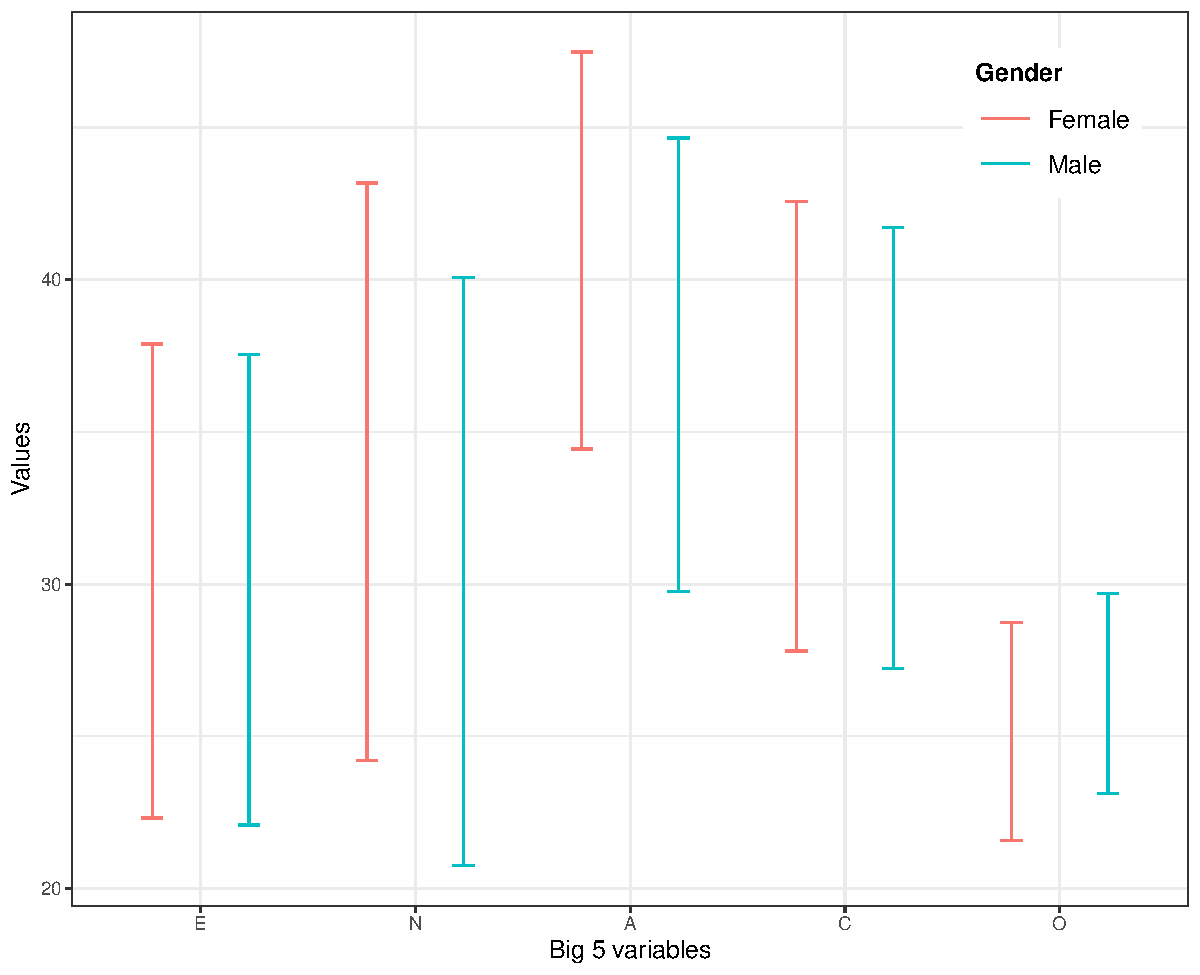
\includegraphics{final_project_files/figure-latex/errorbars-1.pdf}
\caption{\label{fig:errorbars}Difference between Males and Females on Big 5 variables}
\end{figure}

\begin{verbatim}
## 
## Note: parallel analysis suggests 7 components.
\end{verbatim}

\begin{figure}
\centering
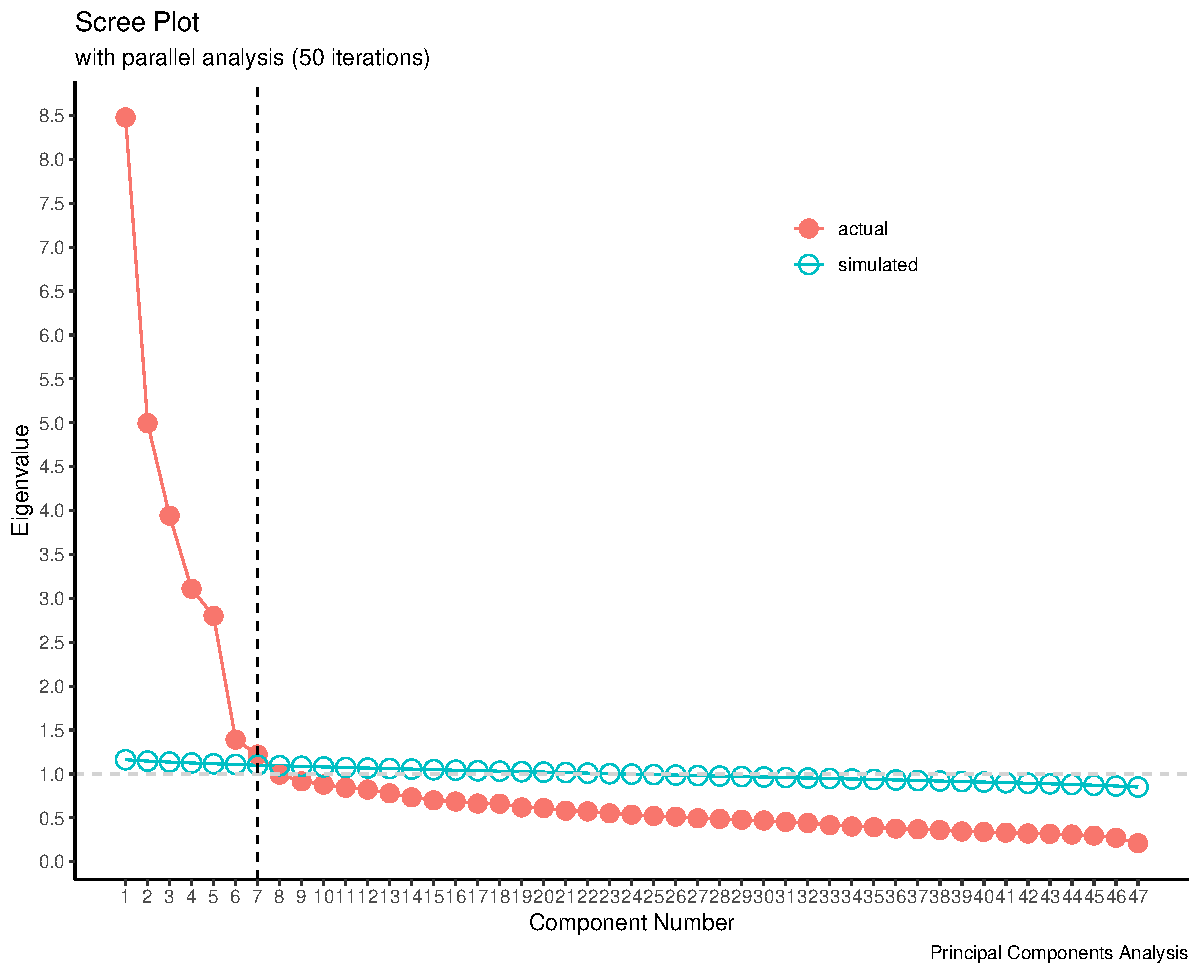
\includegraphics{final_project_files/figure-latex/parallel-analysis-1.pdf}
\caption{\label{fig:parallel-analysis}Parallel analysis}
\end{figure}

\begin{table}[tbp]

\begin{center}
\begin{threeparttable}

\caption{\label{tab:varimaxTable}Varimax rotation loadings matrix}

\tiny{

\begin{tabular}{cccccccc}
\toprule
Items & \multicolumn{1}{c}{RC1} & \multicolumn{1}{c}{RC2} & \multicolumn{1}{c}{RC4} & \multicolumn{1}{c}{RC3} & \multicolumn{1}{c}{RC5} & \multicolumn{1}{c}{RC7} & \multicolumn{1}{c}{RC6}\\
\midrule
E4r & 0.81 & -0.11 & 0.07 & 0.06 & -0.03 & -0.02 & 0.09\\
E5 & 0.77 & -0.08 & 0.23 & 0.07 & 0.08 & 0.02 & -0.07\\
E2 & -0.76 & -0.03 & -0.12 & -0.01 & -0.01 & 0.05 & -0.09\\
E7 & 0.76 & -0.12 & 0.17 & 0.03 & 0.01 & 0.04 & -0.12\\
E10r & 0.75 & -0.16 & 0.07 & 0.04 & -0.02 & -0.02 & 0.10\\
E1 & 0.74 & -0.05 & 0.05 & 0.00 & 0.03 & 0.09 & -0.19\\
E9 & 0.71 & -0.06 & -0.03 & -0.04 & 0.09 & 0.12 & -0.07\\
E3 & 0.68 & -0.28 & 0.25 & 0.11 & 0.05 & -0.01 & -0.15\\
E6r & 0.66 & -0.05 & 0.16 & 0.04 & 0.15 & 0.04 & 0.23\\
E8r & 0.65 & -0.02 & -0.07 & -0.08 & -0.03 & 0.07 & 0.09\\
N6 & -0.06 & 0.79 & 0.01 & -0.08 & -0.07 & -0.01 & -0.10\\
N8 & -0.02 & 0.77 & -0.07 & -0.14 & -0.05 & 0.10 & -0.08\\
N1 & -0.09 & 0.76 & 0.09 & -0.01 & -0.06 & -0.09 & 0.04\\
N9 & -0.05 & 0.74 & -0.19 & -0.04 & 0.02 & -0.02 & -0.13\\
N7 & -0.01 & 0.74 & -0.07 & -0.15 & -0.03 & 0.11 & -0.10\\
N3 & -0.13 & 0.69 & 0.17 & 0.04 & 0.03 & -0.06 & -0.01\\
N10 & -0.27 & 0.68 & -0.05 & -0.17 & -0.01 & 0.03 & 0.14\\
N2r & -0.05 & 0.64 & -0.04 & 0.06 & -0.08 & -0.18 & 0.34\\
N5 & -0.07 & 0.60 & -0.02 & -0.07 & -0.13 & 0.01 & -0.20\\
N4r & -0.20 & 0.53 & 0.01 & -0.13 & -0.06 & 0.01 & 0.29\\
A4 & 0.02 & 0.04 & 0.82 & 0.03 & 0.00 & 0.05 & -0.04\\
A9 & 0.08 & 0.09 & 0.75 & 0.04 & 0.04 & 0.10 & -0.09\\
A5r & 0.14 & 0.01 & 0.71 & 0.00 & -0.02 & -0.03 & 0.18\\
A6 & -0.02 & 0.12 & 0.69 & 0.01 & -0.09 & 0.07 & -0.17\\
A7r & 0.32 & -0.08 & 0.68 & 0.00 & -0.02 & 0.00 & 0.17\\
A8 & 0.12 & -0.06 & 0.67 & 0.09 & 0.08 & 0.02 & -0.12\\
A2 & 0.36 & -0.07 & 0.59 & -0.03 & 0.08 & 0.02 & 0.01\\
A1r & 0.05 & 0.00 & 0.56 & 0.03 & -0.01 & -0.08 & 0.32\\
A3r & -0.13 & -0.25 & 0.46 & 0.22 & -0.13 & 0.00 & 0.15\\
A10 & 0.35 & -0.20 & 0.45 & 0.10 & 0.14 & 0.11 & -0.24\\
C6r & 0.02 & -0.15 & -0.02 & 0.73 & -0.15 & 0.04 & 0.16\\
C5 & 0.08 & -0.09 & 0.06 & 0.72 & -0.03 & 0.02 & -0.12\\
C2r & -0.03 & -0.09 & -0.07 & 0.71 & -0.25 & 0.09 & 0.12\\
C9 & 0.06 & 0.04 & 0.09 & 0.65 & 0.12 & -0.10 & -0.16\\
C7 & -0.05 & 0.10 & 0.03 & 0.65 & 0.17 & -0.07 & -0.11\\
C4r & 0.07 & -0.35 & 0.05 & 0.64 & -0.04 & 0.01 & 0.10\\
C1 & 0.00 & -0.09 & 0.00 & 0.61 & 0.31 & -0.08 & -0.10\\
C8r & 0.08 & -0.20 & 0.15 & 0.52 & 0.13 & -0.07 & 0.20\\
C3 & -0.06 & -0.01 & 0.08 & 0.43 & 0.42 & 0.05 & -0.10\\
O7 & 0.07 & -0.16 & 0.00 & 0.07 & 0.70 & 0.06 & 0.05\\
O1 & 0.05 & -0.03 & -0.04 & -0.05 & 0.62 & 0.12 & 0.27\\
O5 & 0.22 & -0.08 & -0.03 & 0.09 & 0.52 & 0.39 & -0.05\\
C10 & -0.01 & -0.01 & 0.04 & 0.45 & 0.50 & -0.05 & -0.10\\
O6 & -0.11 & 0.05 & -0.09 & 0.02 & -0.09 & -0.81 & -0.13\\
O3 & 0.06 & 0.09 & 0.07 & -0.10 & 0.17 & 0.80 & 0.02\\
O4r & 0.03 & -0.09 & 0.10 & -0.10 & 0.30 & 0.37 & 0.53\\
O2r & 0.05 & -0.20 & -0.01 & -0.05 & 0.46 & 0.30 & 0.52\\
\bottomrule
\addlinespace
\end{tabular}

}

\begin{tablenotes}[para]
\normalsize{\textit{Note.} E = Extraversion, N = Neuroticism, A = Agreeableness, C = Conscientiousness, O = Openness/Intellect}
\end{tablenotes}

\end{threeparttable}
\end{center}

\end{table}

\begin{table}[tbp]

\begin{center}
\begin{threeparttable}

\caption{\label{tab:obliminTable}Oblimin rotation loadings matrix}

\tiny{

\begin{tabular}{cccccccc}
\toprule
Items & \multicolumn{1}{c}{TC1} & \multicolumn{1}{c}{TC2} & \multicolumn{1}{c}{TC4} & \multicolumn{1}{c}{TC3} & \multicolumn{1}{c}{TC5} & \multicolumn{1}{c}{TC7} & \multicolumn{1}{c}{TC6}\\
\midrule
E4r & 0.81 & -0.20 & 0.16 & 0.07 & 0.04 & 0.05 & 0.05\\
E5 & 0.79 & -0.18 & 0.32 & 0.08 & 0.16 & 0.10 & -0.09\\
E7 & 0.78 & -0.21 & 0.26 & 0.04 & 0.08 & 0.11 & -0.15\\
E2 & -0.76 & 0.06 & -0.20 & -0.02 & -0.06 & -0.03 & -0.05\\
E10r & 0.76 & -0.24 & 0.15 & 0.07 & 0.04 & 0.05 & 0.07\\
E1 & 0.74 & -0.13 & 0.13 & -0.01 & 0.09 & 0.15 & -0.22\\
E3 & 0.72 & -0.37 & 0.34 & 0.14 & 0.14 & 0.05 & -0.16\\
E9 & 0.71 & -0.14 & 0.05 & -0.05 & 0.13 & 0.20 & -0.08\\
E6r & 0.69 & -0.14 & 0.23 & 0.05 & 0.19 & 0.14 & 0.21\\
E8r & 0.64 & -0.08 & 0.00 & -0.08 & -0.01 & 0.13 & 0.06\\
N6 & -0.13 & 0.80 & -0.02 & -0.17 & -0.11 & -0.04 & -0.14\\
N8 & -0.10 & 0.78 & -0.10 & -0.23 & -0.11 & 0.08 & -0.11\\
N1 & -0.16 & 0.76 & 0.06 & -0.09 & -0.10 & -0.12 & 0.00\\
N9 & -0.14 & 0.75 & -0.22 & -0.14 & -0.02 & -0.04 & -0.16\\
N7 & -0.09 & 0.75 & -0.10 & -0.24 & -0.09 & 0.10 & -0.13\\
N10 & -0.34 & 0.71 & -0.10 & -0.24 & -0.11 & 0.01 & 0.13\\
N3 & -0.17 & 0.69 & 0.14 & -0.03 & 0.01 & -0.09 & -0.03\\
N2r & -0.11 & 0.65 & -0.05 & 0.01 & -0.12 & -0.21 & 0.28\\
N5 & -0.14 & 0.62 & -0.05 & -0.14 & -0.16 & -0.03 & -0.23\\
N4r & -0.25 & 0.55 & -0.03 & -0.16 & -0.15 & 0.00 & 0.27\\
A4 & 0.10 & 0.01 & 0.82 & 0.06 & 0.03 & 0.05 & -0.01\\
A9 & 0.14 & 0.05 & 0.76 & 0.06 & 0.08 & 0.10 & -0.06\\
A5r & 0.20 & -0.03 & 0.72 & 0.04 & -0.01 & 0.00 & 0.20\\
A7r & 0.39 & -0.13 & 0.71 & 0.05 & 0.00 & 0.04 & 0.18\\
A6 & 0.03 & 0.10 & 0.68 & 0.03 & -0.06 & 0.05 & -0.16\\
A8 & 0.19 & -0.10 & 0.68 & 0.11 & 0.14 & 0.03 & -0.10\\
A2 & 0.42 & -0.13 & 0.62 & -0.01 & 0.10 & 0.08 & 0.03\\
A1r & 0.11 & -0.02 & 0.57 & 0.07 & -0.01 & -0.06 & 0.33\\
A10 & 0.41 & -0.26 & 0.49 & 0.12 & 0.22 & 0.14 & -0.22\\
A3r & -0.07 & -0.26 & 0.46 & 0.28 & -0.06 & -0.05 & 0.14\\
C6r & 0.03 & -0.19 & 0.04 & 0.76 & 0.06 & -0.08 & 0.07\\
C2r & -0.03 & -0.12 & -0.01 & 0.74 & -0.04 & -0.06 & 0.02\\
C5 & 0.09 & -0.14 & 0.12 & 0.72 & 0.19 & -0.09 & -0.19\\
C4r & 0.11 & -0.40 & 0.11 & 0.68 & 0.16 & -0.07 & 0.04\\
C9 & 0.07 & -0.01 & 0.14 & 0.62 & 0.32 & -0.17 & -0.21\\
C7 & -0.04 & 0.05 & 0.07 & 0.61 & 0.35 & -0.14 & -0.16\\
C1 & 0.02 & -0.15 & 0.05 & 0.58 & 0.48 & -0.11 & -0.11\\
C8r & 0.12 & -0.25 & 0.20 & 0.54 & 0.26 & -0.10 & 0.17\\
O7 & 0.12 & -0.21 & 0.01 & 0.03 & 0.70 & 0.19 & 0.14\\
C10 & 0.02 & -0.06 & 0.07 & 0.39 & 0.61 & -0.02 & -0.08\\
O1 & 0.08 & -0.06 & -0.03 & -0.10 & 0.56 & 0.26 & 0.34\\
O5 & 0.25 & -0.14 & 0.00 & 0.04 & 0.56 & 0.48 & 0.00\\
C3 & -0.03 & -0.05 & 0.10 & 0.38 & 0.53 & 0.05 & -0.08\\
O3 & 0.08 & 0.06 & 0.07 & -0.13 & 0.16 & 0.83 & 0.05\\
O6 & -0.15 & 0.08 & -0.11 & 0.01 & -0.11 & -0.82 & -0.14\\
O2r & 0.11 & -0.23 & 0.00 & -0.05 & 0.40 & 0.42 & 0.58\\
O4r & 0.07 & -0.12 & 0.10 & -0.09 & 0.23 & 0.45 & 0.58\\
\bottomrule
\addlinespace
\end{tabular}

}

\begin{tablenotes}[para]
\normalsize{\textit{Note.} E = Extraversion, N = Neuroticism, A = Agreeableness, C = Conscientiousness, O = Openness/Intellect}
\end{tablenotes}

\end{threeparttable}
\end{center}

\end{table}

\hypertarget{results}{%
\section{Results}\label{results}}

Table~\ref{tab:descriptiveTable} displays a summary of differences between males and females and Chronbach's alpha value for all Big 5 variables. There is a significant difference in all the variables for males and females except for Extraversion in this sample. We took a closer look at the error bars to see if there is any overlap. Figure~\ref{fig:errorbars} indicates a very high overlap for genders across Big 5 variables with an almost exact range for Extraversion. This indicates that there is not much difference in the levels of Big 5 in males and females in this sample. All the alpha values seem reasonably acceptable except for a low value for Openness.
Parallel analysis (Horn's method) suggested 7 factors to be retained as seen in Figure~\ref{fig:parallel-analysis}. The seven factor solution was rotated using varimax and oblimin rotations. An examination of loadings matrix for varimax rotation Table~\ref{tab:varimaxTable} and structure matrix for oblimin rotation Table~\ref{tab:obliminTable} indicate a clear emergence of the first three factors -Extraversion, Neuroticism, Agreeableness - indicating the respective items with highest loading on those factors. The last two factors - Conscientiousness and Openness - tend to split into multiple factors.

\hypertarget{discussion}{%
\section{Discussion}\label{discussion}}

Althought the t-test indicated significant differences overlaps seen in the errorbars indicate that no main differences can be seen in the plots. Openness and conscientiousness split into more factors which indicate a rather interesting groupings of variables into factors for this data. One could further look at inter item consistency values for these groups of 7 factors for the data.

\newpage

\hypertarget{references}{%
\section{References}\label{references}}

\begingroup
\setlength{\parindent}{-0.5in}
\setlength{\leftskip}{0.5in}

\hypertarget{refs}{}
\leavevmode\hypertarget{ref-R-papaja}{}%
Aust, F., \& Barth, M. (2020). \emph{papaja: Create APA manuscripts with R Markdown}. Retrieved from \url{https://github.com/crsh/papaja}

\leavevmode\hypertarget{ref-R-GPArotation}{}%
Bernaards, C. A., \& I.Jennrich, R. (2005). Gradient projection algorithms and software for arbitrary rotation criteria in factor analysis. \emph{Educational and Psychological Measurement}, \emph{65}, 676--696.

\leavevmode\hypertarget{ref-R-gapminder}{}%
Bryan, J. (2017). \emph{Gapminder: Data from gapminder}. Retrieved from \url{https://CRAN.R-project.org/package=gapminder}

\leavevmode\hypertarget{ref-R-rio}{}%
Chan, C.-h., Chan, G. C., Leeper, T. J., \& Becker, J. (2018). \emph{Rio: A swiss-army knife for data file i/o}.

\leavevmode\hypertarget{ref-R-paran}{}%
Dinno, A. (2018). \emph{Paran: Horn's test of principal components/factors}. Retrieved from \url{https://CRAN.R-project.org/package=paran}

\leavevmode\hypertarget{ref-R-janitor}{}%
Firke, S. (2020). \emph{Janitor: Simple tools for examining and cleaning dirty data}. Retrieved from \url{https://CRAN.R-project.org/package=janitor}

\leavevmode\hypertarget{ref-R-purrr}{}%
Henry, L., \& Wickham, H. (2020). \emph{Purrr: Functional programming tools}. Retrieved from \url{https://CRAN.R-project.org/package=purrr}

\leavevmode\hypertarget{ref-R-ggpubr}{}%
Kassambara, A. (2020a). \emph{Ggpubr: 'Ggplot2' based publication ready plots}. Retrieved from \url{https://CRAN.R-project.org/package=ggpubr}

\leavevmode\hypertarget{ref-R-rstatix}{}%
Kassambara, A. (2020b). \emph{Rstatix: Pipe-friendly framework for basic statistical tests}. Retrieved from \url{https://CRAN.R-project.org/package=rstatix}

\leavevmode\hypertarget{ref-R-here}{}%
Müller, K. (2017). \emph{Here: A simpler way to find your files}. Retrieved from \url{https://CRAN.R-project.org/package=here}

\leavevmode\hypertarget{ref-R-tibble}{}%
Müller, K., \& Wickham, H. (2020). \emph{Tibble: Simple data frames}. Retrieved from \url{https://CRAN.R-project.org/package=tibble}

\leavevmode\hypertarget{ref-R-base}{}%
R Core Team. (2019). \emph{R: A language and environment for statistical computing}. Vienna, Austria: R Foundation for Statistical Computing. Retrieved from \url{https://www.R-project.org/}

\leavevmode\hypertarget{ref-R-psych}{}%
Revelle, W. (2020). \emph{Psych: Procedures for psychological, psychometric, and personality research}. Evanston, Illinois: Northwestern University. Retrieved from \url{https://CRAN.R-project.org/package=psych}

\leavevmode\hypertarget{ref-R-MASS}{}%
Venables, W. N., \& Ripley, B. D. (2002). \emph{Modern applied statistics with s} (Fourth). New York: Springer. Retrieved from \url{http://www.stats.ox.ac.uk/pub/MASS4}

\leavevmode\hypertarget{ref-R-ggplot2}{}%
Wickham, H. (2016). \emph{Ggplot2: Elegant graphics for data analysis}. Springer-Verlag New York. Retrieved from \url{https://ggplot2.tidyverse.org}

\leavevmode\hypertarget{ref-R-forcats}{}%
Wickham, H. (2019a). \emph{Forcats: Tools for working with categorical variables (factors)}. Retrieved from \url{https://CRAN.R-project.org/package=forcats}

\leavevmode\hypertarget{ref-R-stringr}{}%
Wickham, H. (2019b). \emph{Stringr: Simple, consistent wrappers for common string operations}. Retrieved from \url{https://CRAN.R-project.org/package=stringr}

\leavevmode\hypertarget{ref-R-tidyr}{}%
Wickham, H. (2020). \emph{Tidyr: Tidy messy data}. Retrieved from \url{https://CRAN.R-project.org/package=tidyr}

\leavevmode\hypertarget{ref-R-tidyverse}{}%
Wickham, H., Averick, M., Bryan, J., Chang, W., McGowan, L. D., François, R., \ldots{} Yutani, H. (2019). Welcome to the tidyverse. \emph{Journal of Open Source Software}, \emph{4}(43), 1686. \url{https://doi.org/10.21105/joss.01686}

\leavevmode\hypertarget{ref-R-usethis}{}%
Wickham, H., \& Bryan, J. (2020). \emph{Usethis: Automate package and project setup}. Retrieved from \url{https://CRAN.R-project.org/package=usethis}

\leavevmode\hypertarget{ref-R-dplyr}{}%
Wickham, H., François, R., Henry, L., \& Müller, K. (2020a). \emph{Dplyr: A grammar of data manipulation}. Retrieved from \url{https://CRAN.R-project.org/package=dplyr}

\leavevmode\hypertarget{ref-R-devtools}{}%
Wickham, H., Hester, J., \& Chang, W. (2020b). \emph{Devtools: Tools to make developing r packages easier}. Retrieved from \url{https://CRAN.R-project.org/package=devtools}

\leavevmode\hypertarget{ref-R-readr}{}%
Wickham, H., Hester, J., \& Francois, R. (2018). \emph{Readr: Read rectangular text data}. Retrieved from \url{https://CRAN.R-project.org/package=readr}

\leavevmode\hypertarget{ref-R-dbplyr}{}%
Wickham, H., \& Ruiz, E. (2019). \emph{Dbplyr: A 'dplyr' back end for databases}. Retrieved from \url{https://CRAN.R-project.org/package=dbplyr}

\leavevmode\hypertarget{ref-R-scales}{}%
Wickham, H., \& Seidel, D. (2019). \emph{Scales: Scale functions for visualization}. Retrieved from \url{https://CRAN.R-project.org/package=scales}

\leavevmode\hypertarget{ref-R-knitr}{}%
Xie, Y. (2015). \emph{Dynamic documents with R and knitr} (2nd ed.). Boca Raton, Florida: Chapman; Hall/CRC. Retrieved from \url{https://yihui.org/knitr/}

\leavevmode\hypertarget{ref-R-tinytex}{}%
Xie, Y. (2019). TinyTeX: A lightweight, cross-platform, and easy-to-maintain latex distribution based on tex live. \emph{TUGboat}, (1), 30--32. Retrieved from \url{http://tug.org/TUGboat/Contents/contents40-1.html}

\endgroup


\end{document}
